\chapter{Contando listas de números}\label{combinatoria:contando_listas_de_numeros}
Ver diapositivas \textit{''Contando listas de numeros``}

\begin{ejemplo}
Cuántos número hay en la siguiente lista?
\[
1,2,3,4,\dots,16,17,18?
\]
Claramente hay 18. Esta es una \textbf{lista fácil de contar }.
\end{ejemplo}

\begin{ejemplo}
	Cuántos número hay en la siguiente lista?
	\[
	1,2,3,4,\dots,16,17,2020?
	\]
	Es una lista facil! hay 2020.
\end{ejemplo}

\begin{tcolorbox}[colback=red!5!white,colframe=red!75!black]
	Usando una variable $n$, tenemos que para cualquier valor que tenga $n$ la cantidad de números en la lista
	\[
	1,2,3,4,\dots,n-2,n-1,n
	\]
	es $n$.
\end{tcolorbox}



\begin{ejemplo}
Cuántos números hay en la sigueinte lista?
\[
7,8,9,10,11,12,13,14,15,16,17,18,19,20,21,22,23,24,25,26,27,28,29
\]
\begin{itemize}
	\item \textbf{Forma 1: }Como son pocos podemos contarlos uno a uno y ver que son 23.
	\item \textbf{Forma 2: } Podremos convertir esta lista en una lista fácil? claro que si!
			\begin{align*}
				7  & 8   &9  &\cdots  &27&28 &29\\
				-6 & -6 &-6 &\cdots &-6 &-6 &-6\\
				\hline \\
				1  &2   &3  &\cdots  &21&22 &23
			\end{align*}
			Al restarle -6 a todos cambió la cantidad de números en la lista? o sigue habiendo la misma cantidad?. Note que al restarle no cambia la cantidad que es lo que nos importa! Entonces en la lista hay 23 números pues la hemos convertido a una lista fácil.
\end{itemize}
\end{ejemplo}

\begin{exer}{\ \\}
	Cuántos números hay en la siguiente lista de números?
	\[21,22,23,\cdots, 98,99,100\]
\end{exer}

\begin{exer}{\ \\}
	Cuántos números hay en la siguiente lista de números?
	\[321,322,323,\cdots, 2018,2019,2020\]
\end{exer}

\begin{exer}\label{ejercicio_cantidad_numeros_en_una_lista}
	\textbf{Avanzado}. Si se tienen dos números cualquiera $a$ y $b$ tal que $b$ es mas grande que $a$, encontrar una fórmula para saber cuántos números hay entre $a$ y $b$ incluyendolos, es decir
	\[
	a,a+1,a+2,\dots, b
	\]	
\end{exer}

\begin{ejemplo}
Cuántos múltiplos de 3 hay entre 62 y 215?
\textbf{Rta: } Escribamos nuestra lista! Donde empieza? donde termina?
\[
63,66,69,\dots , 207, 210,213
\]
Será que restandole algo quedará una lista fácil? \textbf{NO}. Pero vemos que la lista va de 3 en 3, entonces dividimos por 3 y  obtenemos la lista
\[
21,2,23,\dots , 69, 70,71
\]
Esta si la podemos volver fácil, restando cuanto? Si, 20.
\[
1,2,3,\dots,49,50,51
\]
Entonces hay 51 números en la lista.
\textbf{Otra solución: } 
Como la lista va de 62 a 215 entonces hay $\frac{215-62}{3}=\frac{153}{3}=51$. Hmm, esto siempre funcionará?
\end{ejemplo}


\begin{exer}
Realizar estos ejercicios de dos formar: primero como la última forma y luego reduciendolos a una lista fácil.
\begin{enumerate}[label=\Alph*)]
	\item Cuantos múltiplos de 10 hay entre 9 y 101?
	\item Cuántos múltiplos de 10 hay entre 11 y 103?
\end{enumerate}
Cuál de los dos métodos funciona siempre?
\end{exer}


\begin{tcolorbox}[colback=red!5!white,colframe=red!75!black]
	\textbf{OJO!} Ver que $\frac{101-9}{10}=\frac{103-11}{10}=9,2$ pero sin embargo en una lista habían 10 y en la otra 9. Luego, no nos debemos confiar de este método.
\end{tcolorbox}

\begin{ejemplo}
Cuántos múltiplos de 5 hay entre 100 y 1000 incluyendolos?
\end{ejemplo}

\begin{tcolorbox}[colback=red!5!white,colframe=red!75!black]
	Para contar elementos de una lista debemos saber cuál es el \textbf{primero} y cuál es el \textbf{último}.	
\end{tcolorbox}

\begin{exer}
	Cuántos múltiplos de 4 hay entre 100 y 2020 incluyendolos?
\end{exer}

\begin{ejemplo}
Cuántos números de 4 dígitos son cubos perfectos?
\end{ejemplo}

\begin{tcolorbox}[colback=white!5!white,colframe=green!50!black]
	Se recomienda para la actividad \ref{ejercicios:part:combinatoria:chp:contando_listas_de_numeros} hacer relevos de forma individual o por parejas.
\end{tcolorbox}


\newpage
\entraAEjercicios{combinatoria:ContandoListasDeNumeros}		
\begin{center}
\vspace{-1cm}
\section{ Ejercicios: Contando listas de números. }\label{ejercicios:part:combinatoria:chp:contando_listas_de_numeros}
\end{center}
	\begin{enumerate}
	\item (p.5 de \cite{Aops_intro_counting_prob}). Cuántos números hay en la siguiente lista 
	\[36,37,38, \dotsi ,92,93 \]
	\item (p.5 de \cite{Aops_intro_counting_prob}). Cuántos números hay en la siguiente lista
	\[4,6,8, \dotsi ,128,130\]
	\item (p.23 de \cite{Aops_intro_counting_prob}). Cuántos números hay en la siguiente lista?
	\[6,10,14,18,\dots, 82,86\]
	\item (p.5 de \cite{Aops_intro_counting_prob}). Cuántos números hay en la siguiente lista
	\[147,144,141, \dotsi ,42,39\]
	\item (p.5 de \cite{Aops_intro_counting_prob}). Cuántos números hay en la siguiente lista
	\[-33,-28,-23, \dotsi ,52,57\]
	\item (p.23 de \cite{Aops_intro_counting_prob}). Cuántos números hay en la siguiente lista?
	\[2{.} 5, 5{.}5, 8{.}5,\dots , 80{.}5, 83{.}5\]
	\item (p.6 de \cite{Aops_intro_counting_prob}). Cuántos múltiplos positivos de 7 son menores que 150?
	\item Cuántos números naturales entre 100 y 10000 son divisibles por 2,3 y 7 al mismo tiempo?
	\item Cúantas potencias de 3 hay entre 90 y 10000?
	\item (p.6 de \cite{Aops_intro_counting_prob}). Cuántos números hay en la siguiente lista
	\[3\frac{2}{3},4\frac{1}{3},5,5\frac{2}{3}, \dotsi ,26\frac{1}{3},27\]
	\item Cuántos números de 4 dígitos son cuadrados perfectos?
	\item (p.6 de \cite{Aops_intro_counting_prob}). \textbf{Wow} Cuántos conjuntos de cuatro números enteros positivos consecutivos hay tales que el producto de ellos es menor que 100000?
		\end{enumerate}

\saleASolution{solution:combinatoria:ContandoListasDeNumeros}

\newpage	

\begin{tcolorbox}[colback=white!5!white,colframe=green!50!black]
	Se recomienda seguir con el capítulo de Sumas: \ref{chapter_sumas} .                                                         
\end{tcolorbox}


\chapter{Principio de Multiplicación}\label{Pmultiplicacion}


\begin{ejemplo}
	Una bandera como la de abajo, quiere ser pintada utilizando dos de los colores que se muestran al lado. ¿De cuántas maneras puede ser pintada la bandera?
	
	\begin{figure}[H]
		\centering
		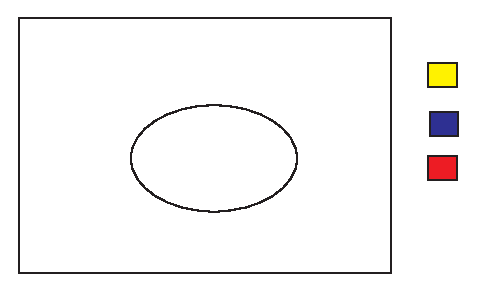
\includegraphics[width=0.6\textwidth]{Combinatoria/imgs/Bandera.eps}
		\caption{Bandera}
		\label{fig:Bandera}
	\end{figure}
	
	\label{Ejemplobandera}
\end{ejemplo}
Antes de mostrar la solución del problema es importante ser ordenados a la hora de contar nuestros casos.
\begin{figure}[H]
	\centering
	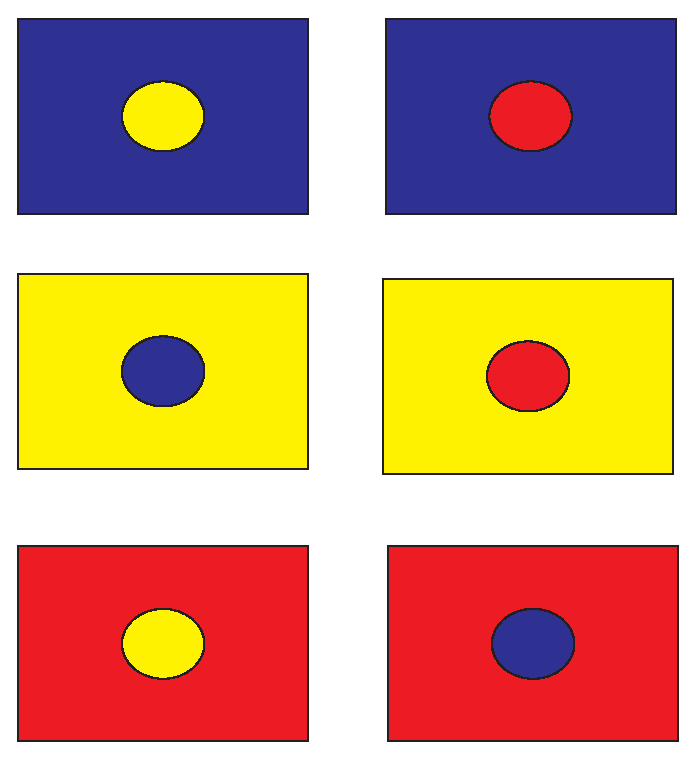
\includegraphics[width=0.4\textwidth]{Combinatoria/imgs/banderasol.eps}
	\caption{Solución \ref{Ejemplobandera}}
	\label{solbandera}
\end{figure}


Para el caso anterior, es útil contar en primer lugar los colores que pueden ir en la parte externa de la figura y después los colores que irán en la parte interna. Para esto puede ser de gran ayuda el \textbf{Diagrama de árbol}.

\begin{figure}[H]
	\centering
	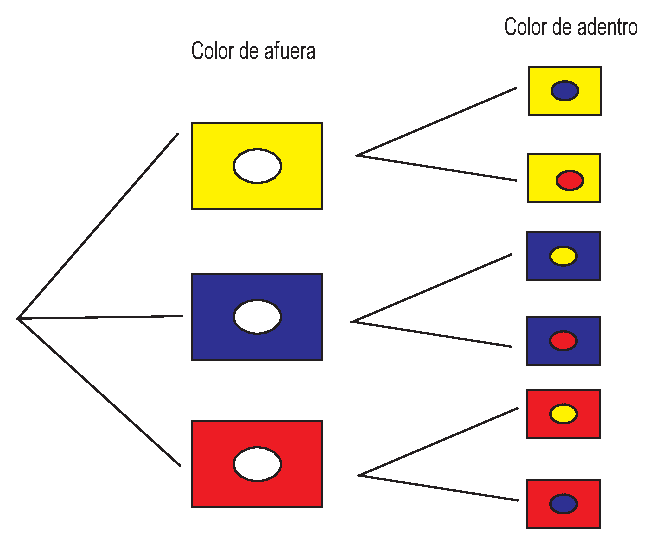
\includegraphics[width=0.5\textwidth]{Combinatoria/imgs/diagramadearbolbandera.eps}
	\caption{Diagrama de Árbol}
	\label{Diagramadearbolbandera}
\end{figure}

Es de notar que al elegir el color externo tenemos 3 opciones y una vez elegido este, quedan 2 opciones para cada uno de los casos, es decir, habrían en total $3\times2=6$ maneras de pintar la bandera.

\begin{ejemplo}
	Y si ahora fueran 4 colores. ¿De cuántas maneras se puede colorear la bandera de manera que se utilicen 2 colores diferentes?.
\end{ejemplo}

\textit{Solución.} Haciendo un diagrama de árbol y usando la misma idea anterior se llega a que habrían $4\times 3$ formas de hacerlo. 

\begin{ejemplo}
	Una bandera como la de abajo, quiere ser pintada utilizando 3 de los 4 colores que se muestran al lado. ¿De cuántas maneras puede ser pintada la bandera?
	\label{ejemplobandera3regiones}
\end{ejemplo}

\begin{figure}[H]
	\centering
	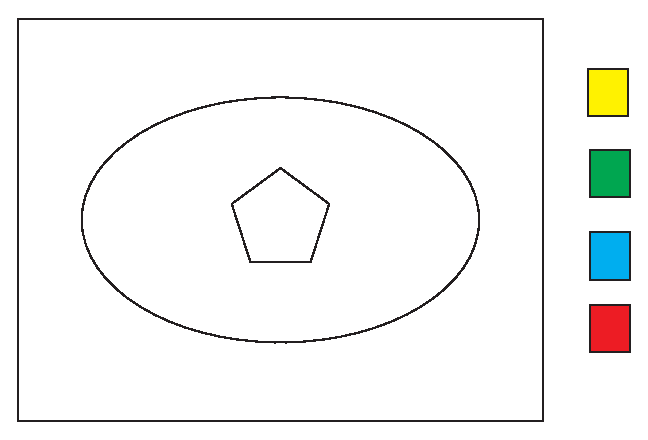
\includegraphics[width=0.4\textwidth]{Combinatoria/imgs/bandera3regiones.eps}
	\caption{Ejemplo \ref{ejemplobandera3regiones}}
	\label{bandera3regiones}
\end{figure}

\textit{Solución.} Si hicieramos el árbol nuevamente, sabemos que al inicio tenemos 4 opciones para elegir el color de la zona externa, luego como ya usamos uno, de cada una de estas ramas tendríamos 3 posibles colores para pintar la zona de la mitad pues ya se usó un color. Es decir, que hasta ahora van $4\times 3=12$ formas distintas. Así que para cada una de estas $12$ ramas quedarán solo 2 colores posibles para pintar la zona interior. Por tanto en total habrían $4\times 3\times 2=24$ opciones.

\begin{ejemplo}
	Un aventurero quiere ir de la ciudad A a la ciudad B pasando por C y usando los caminos señalados en la figura. ¿Cuántos caminos distintos puede tomar el aventurero para llegar a la ciudad B?\\
	\label{EjemplociudadAaC}
\end{ejemplo}

\begin{figure}[H]
	\centering
	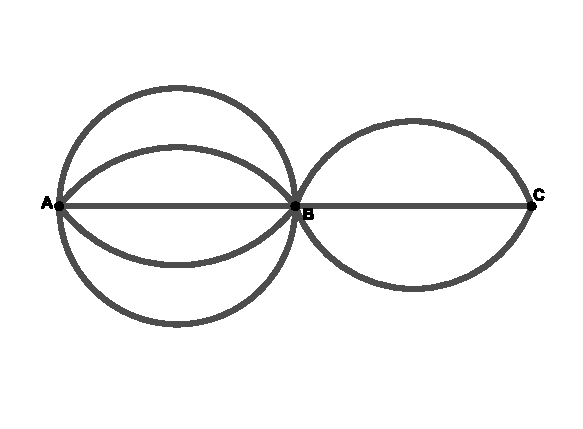
\includegraphics[width=0.6\textwidth]{Combinatoria/imgs/CAMINOSAaC.eps}
	\caption{Ejemplo \ref{EjemplociudadAaC}}
	\label{caminosAaC}
\end{figure}

\textit{Solución. }En este caso trataremos de contar de una forma distinta. Es útil nombrar los caminos como sigue

\begin{figure}[H]
	\centering
	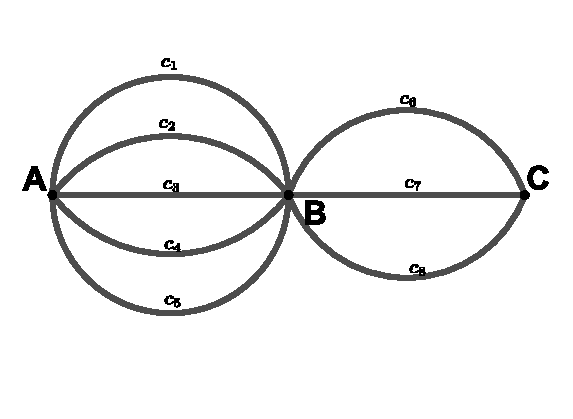
\includegraphics[width=0.6\textwidth]{Combinatoria/imgs/CAMINOSAaCrotulados.eps}
	\caption{Ejemplo \ref{EjemplociudadAaC} con caminos nombrados}
	\label{caminosAaCrotulados}
\end{figure}

En la siguiente tabla encontramos en la parte superior de la tabla están los caminos de la ciudad A a B, y en la parte vertical de la tabla los caminos posibles de B a C.


\begin{center}
	\begin{table}[H]
		\centering
		\begin{tabular}{|c|c|c|c|c|c|}
			\hline
			& $c_1$        & $c_2$        & $c_3$        & $c_4$        & $c_5$        \\ \hline
			$c_6$ & $c_1$ y $c_6$ & $c_2$ y $c_6$ & $c_3$ y $c_6$ & $c_4$ y $c_6$ & $c_5$ y $c_6$ \\ \hline
			$c_7$ & $c_1$ y $c_7$ & $c_2$ y $c_7$ & $c_3$ y $c_7$ & $c_4$ y $c_7$ & $c_5$ y $c_7$ \\ \hline
			$c_8$ & $c_1$ y $c_8$ & $c_2$ y $c_8$ & $c_3$ y $c_8$ & $c_4$ y $c_8$ & $c_5$ y $c_8$ \\ \hline
		\end{tabular}
		\caption{Caminos posibles para ir de A a C.}
		\label{tablacaminosAaC}
	\end{table}
\end{center}


En la tabla se ve que hay 15 caminos para ir de A a B y cada uno de ellos es distinto.
\vspace{0.3cm}

No siempre es útil utilizar este tipo de tablas o diagramas de árbol. Es por eso que debemos ayudarnos de un método mas sencillo.

\begin{defi}
	Cuándo al tratar de contar casos nos enfrentamos ante varias decisiones, es cuando usamos lo que se conoce como \textbf{Principio de Multiplicación}. Y lo que este dice, es que simplemente se multiplicar la cantidad de decisiones una tras otra. Para así, hallar la cantidad de todas las posibles opciones.
\end{defi}

\begin{ejemplo}
	La bandera de abajo debe ser pintada con 3 colores de tal manera que los colores que estén adyacentes sean distintos. Los 4 colores a la derecha son los que pueden ser usados. ¿De cuántas maneras puede ser pintada la bandera? 
\end{ejemplo}
\vspace{2cm}

(***Bandera de 3 franjas como de Colombia***)

\vspace{2cm}

\textit{Solución.} En primer lugar, hay 4 formas de pintar la franja de arriba. Luego de pintada esta, hay 3 formas de pintar la de la mitad, pues este color debe ser distinto al de arriba. Y para la franja de abajo, se podría pensar que hay 2 opciones porque no puedo usar el color del medio, pero note que podría volver a usar el color de la franjsa de arriba. Así, que para la de abajo hay 3 opciones. Usando el \textit{Principio de Multiplicación} habrían $4\times 3\times 3=24$ formas de pintar la bandera.

\begin{problem}
	Marta va a ir a una fiesta y deberá vestirse con un sombrero, un vestido y unos tacones. Ella tiene 3 sombreros distintos, tiene un vestido rojo y otro negro, y además tiene dos tacones, unos altos y otros bajos. ¿De cuántas maneras se podrá vestir Marta?\\
	a) Hacer un diagrama de árbol.\\
	b) Luego usar el principio de multiplicación y comparar.
\end{problem}

\begin{problem}
	¿Cuántos hay cuyos dígitos son todos distintos?
	\label{problema3digitosdistintos}
\end{problem}

\begin{ejemplo}
	El código binario utiliza únicamente los dígitos 1 y 0 para formar números. Por ejemplo, el 1101001 es un número binario de 7 dígitos. ¿Cuántos números binarios hay tales que tengan con máximo 4 dígitos?
\end{ejemplo}

\textit{Solución.} De longitud uno hay 2 números, el 1 y el 0. De longitud dos hay $2\times 2 = 4$. De longitud tres hay $2\times 2\times 2=8$. Y de longitud cuatro hay $2\times 2\times 2\times 2=16$ números. Así que en total hay $2+4+8+16=30$ números binarios tales que tienen como máximo 4 dígitos.

\section*{Postura Combinatorica.}
\begin{itemize}
	\item En los ejemplos trabajados hasta ahora y en general, es importante tomar una postura siempre del lado del objeto problema. Por ejemplo, al colorear la bandera, ponerse en el lado de quien pinta la bandera y ver que decisiones tiene que ir tomando esta persona.
	\item Las etapas del problema deben ser identificadas, por ejemplo al colorear la bandera fue útil decidir primero pintar el exterior y así hasta el interior. O en el caso de los número binarios fue necesario primero ver los números de 1 dígito, luego los de 2, después los de 3 y por último los de 4 dígitos.
	\item Por último saber ver cuál es la decisión más importante y aquella que tenga mas condiciones, por ejemplo en el problema de los números de 3 dígitos es importante saber que el primero dígito no puede ser cero. Así que debemos empezar a contar los casos por la decisión de poner el primer número.
\end{itemize}

\begin{ejemplo}
	¿Cuántos números pares de tres dígitos se pueden formar de tal manera que todos los dígitos sean distintos?
\end{ejemplo}

\textit{Solución 1.} Poniéndonos en el lugar del número, sabemos que este debe terminar en 0,2,4,6,8. Pero también debemos tener en cuenta que el 0 no puede ir en la primera posición. Así que tenemos varias condiciones para nuestro problema y es útil atacarlo por partes. El primer caso es cuando colocamos el 0 en la última posición, pues ahora para el primer dígito solo tendría 9 opciones. Pero si no se coloca el 2,4,6 0 8 en la última posición, se tendrán 8 opciones para el primer dígito, pues no puede ser 0 ni tampoco el que ya fue usado en la última posición. Es decir, el problema cambió, pues si pensamos en \ref{problema3digitosdistintos} allí las decisiones no cambiaban, en cambio acá las decisiones cambian cuando coloco o no coloco el 0 de último. Por tanto debemos contar ambos casos por aparte. Para el primero habrían $9\times 8 \times 1=72$ formas, pues como dijimos hay 9 formas para poner el primer número, 8 formas para el segundo porque no podemos usar el de la primera posición y 1 manera para el último, pues este dijimos que iba a ser 0. En el segundo caso habrían $8\times 8\times 4= 256$, pues para la primera posición dijimos que pueden ir 8, para la segunda se pensaría que pueden ir 7 pero se debe tener en cuenta que ahora si se puede usar el 0, por eso habrían 8 opciones para el segundo lugar y por último habrían 4 opciones para el último puesto (2,4,6,8). Así ya contamos ambos casos y se tendría que la cantidad total sería $72+256=328$.

\textit{Solución 2.} Otra manera de atacar el problema podría ser contar muchos casos y luego restar los que no funcionan. Por ejemplo contar todos los números que terminan en 0,2,4,6 o 8 y restar cuáles de estos números empiezan en 0. Entonces, para contar todos los que terminan en 0,2,4,6 o 8 sabemos que habrían 5 opciones para la última posición (0,2,4,6,8), luego habrían 9 opciones para la primera posición (Pues no se puede repetir el que ya se puso de último) y para la posición del medio habrían 8. Es decir, habrían $9\times 8\times 5=360$ maneras de formar números de 3 dígitos que terminen en 0,2,4,6 o 8. Pero de estos, hay casos que no sirven y son los que empiezan en 0. Para la última posición habrían 4 opciones (2,4,6,8. Ya que el 0 va a ir en la primera), para la primera posición hay 1 opción (Pues va el 0) y para la segunda 8 opciones (pues ya se usaron dos números). Así que hay $1\times 8\times 4=32$ números pares de tres dígitos que empiezan en 0. Así que restando estos de los anteriores tendríamos $360-32=328$.

\begin{ejemplo}
	¿De cuántas formas pueden hacer una fila 6 personas distintas?
\end{ejemplo}
\textit{Solución.} $6\times5\times4\times3\times2\times1$.
\vspace{0.2cm}

\begin{defi}
	Para evitar escribir $6\times5\times4\times3\times2\times1$ se usa $6!$ y se lee "\textit{seis factorial}". Es decir $n\times (n-1) \times (n-2) \cdots \times 3 \times 2\times 1 = n!$ y se lee "n factorial".
\end{defi}

\subsection*{\centering Práctica.}
Hallar otra expresión para cada una de las siguientes:
\begin{enumerate}[label=(\alph*)]
	\item $\frac{10!}{6!}$
	\item $\frac{5!4!}{6!}$
	\item $10!+11!$
	\item $\frac{6!+7!}{2!3!4!}$
	\item $n!(n^2 + 3n+2)$
	\item $\frac{(2n)!-(2n-1)!}{(2n)!-(n-1)!}$
	\item $\frac{(2n)!}{1\times 2\times 3\cdots \times (2n-1)}$
\end{enumerate}

\newpage
\begin{center}
	\vspace{-1cm}
	\section{ Ejercicios: Principio de multiplicación}\label{ejercicios:combinatoria:contandoListasDeNumeros}
\end{center}	
\begin{enumerate}
	\item ¿Cuántos números pares de tres dígitos pueden ser formados utilizando el 2,3,4 y 5 con la condición de que solo se puede usar máximo una vez cada dígito? (Ejercicio 1 de \textit{Primera Capacitación, básico, 2018, Principio de multiplicidad}).
	\item 
	\begin{enumerate}
		\item ¿Cuántos números naturales de tres cifras se pueden formar con los dígitos 2, 3, 4, 5, 6, 7, 8?
		\item ¿Cuántos números naturales de tres cifras \textbf{diferentes} se pueden formar con los dígitos 2, 3, 4, 5, 6, 7, 8? (Ejercicio 2 de \textit{Primera Capacitación, básico, 2018, Principio de multiplicidad}).
	\end{enumerate}
	\item ¿Cuántas palabras de tres letras se pueden formar únicamente usando las siguientes dos letras:\textit{a} y \textit{b}? .
	\item ¿De cuántas maneras se pueden sentar 5 personas en cinco puestos numerados del 1 al 5?
	\item Se desea ubicar 5 niños y 6 niñas en una fila de modo que los niños ocupen los lugares pares. ¿De cuántas formas puede hacerse? (Ejercicio 9 de \textit{Primera Capacitación, básico, 2018, Principio de multiplicidad}).
	\item Juan, Carlos, Tomás, María y José van al cine y les fueron asignadas cinco sillas consecutivas. ¿De cuántas formas se pueden sentar, si Juan y María están uno al lado del otro y nadie, además de María, está junto a Juan? (Ejercicio 10 de \textit{Primera Capacitación, básico, 2018, Principio de multiplicidad}).
	\item \label{problema_camino_flechas} De cuántas formas se puede ir del punto $A$ a $B$? (Ver figura \ref{problema7principiomultiplicacion})
	
	\begin{figure}[b]
		\centering
		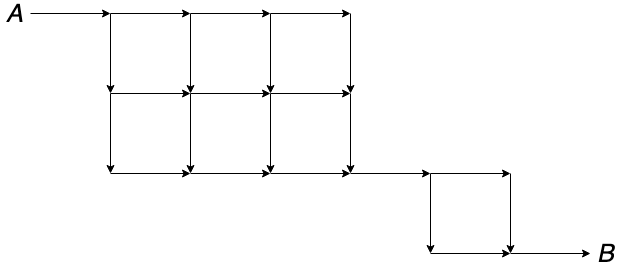
\includegraphics[width=0.7\linewidth]{Combinatoria/imgs/problema7Principiomultiplicacion}
		\caption{Ver problema \ref{problema_camino_flechas}}
		\label{problema7principiomultiplicacion}
	\end{figure}
	
	\item Las placas de los carros son formadas por 3 letras (En un abecedario de 27 letras) y 3 dígitos. ¿Cuántas placas se pueden formar en total?
	\item Un grupo de 4 estudiantes (Alejandro, Blanca, Carlos, Daniela) quieren elegir el presidente y vicepresidente del salón. (Tomado de \cite{Contagem_e_probabilidade})
	\begin{enumerate}
		\item Haga una lista de todas las posibles formas de elegir al presidente(a) y vicepresidente(a). 
		\item ¿Cómo utilizaría el Principio de Multiplicación para contar?
	\end{enumerate} 
	\item \textbf{... ten cuidado.} \label{Problema_bandera_6colores} De cuántas formas se puede pintar la bandera (de la figura \ref{bandera6coloresprincipiomultiplicacion}) usando los seis colores de modo que las secciones adyacentes estén pintadas de diferente color?
	
	\begin{figure}
		\centering
		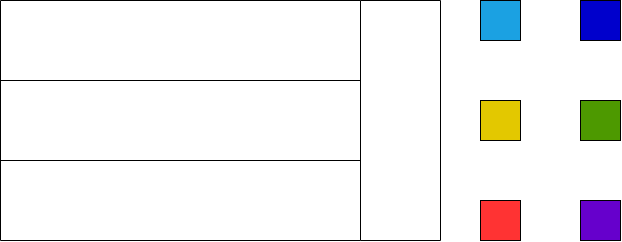
\includegraphics[width=0.7\linewidth]{Combinatoria/imgs/bandera_6_colores_Principiomultiplicacion}
		\caption{Ver Problema \ref{Problema_bandera_6colores}.}
		\label{bandera6coloresprincipiomultiplicacion}
	\end{figure}
	\item \textbf{... ten cuidado.} Se tiene un circulo dividido en 4 partes iguales. Martín tiene 5 colores en su mano y quiere saber de cuántas formas puede colorear el circulo con la condición de que las partes del circulo que comparten un lado no queden con el mismo color. (\textit{Cap 1, ejercicio 7 de }\cite{Contagem_e_probabilidade})
	\item Un examen consta de 8 preguntas, cada una de ellas con 5 respuestas múltiples (A,B,C,D y E). 
	\begin{enumerate}
		\item ¿Cuántos resultados distintos puede tener el examen?
		\item ¿En cuántos de estos resultados aparece solo una pregunta respondida con la letra A?
		\item ¿En cuántos de los resultados \textbf{no} aparece ninguna pregunta respondida con la letra A?
	\end{enumerate}
	\item \label{subconjuntos1,2,3}Dado el conjunto $\{ 1,2,3 \}$.
	\begin{enumerate}
		\item Haga una lista con todos los subconjuntos.
		\item ¿Cuántos subconjuntos hay?
	\end{enumerate}
	\item ¿Cuántos subconjuntos tiene el conjunto $\{1,2,3,\ldots ,n \}$? (Ver \ref{subconjuntos1,2,3})
	\item (\textit{Cap 1, ejercicio 13 de }\cite{Contagem_e_probabilidade})
	\begin{enumerate}
		\item ¿De cuántas maneras se puede formar una palabra de 6 letras (El abecedario tiene 27 letras) si la letra A debe ir en la palabra pero no puede estar en el primer lugar?
		\item ¿Y si la palabra no puede tener letras repetidas?
	\end{enumerate}
	\item Se escriben los números enteros del1 hasta el 2222. (\textit{Cap 1, ejercicio 16 de }\cite{Contagem_e_probabilidade})
	\begin{enumerate}
		\item Cuántas veces está escrito el dígito 0?
		\item En cúantos números aparece el dígito 0? 
	\end{enumerate}
	\item Cuántos enteros positivos de 4 dígitos hay en los cuales aparece el dígito 5? (\textit{Cap 1, ejercicio 17 de }\cite{Contagem_e_probabilidade})
	\item \textit{Teniendo 4 colores disponibles, de cúantas maneras se puede pintar una bandera de tres franjas si las franjas adyacentes deben ser de distinto color?}. Un estudiante da la siguiente solución: "Primero, voy a pintar las franjas extremas; para cada una, tengo 4 posibilidades de escoger. Después, yo pinto la franja central; como tiene que tener color diferente a sus dos franjas distintas, yo puedo escoger su color de apenas 2 formas. Luego, el número total de formas de pintar la bandera es $4\times 4\times 2=32$". La solución es corecta? Si no es correcta, dónde está el error? (\textit{Cap 1, ejercicio 19 de }\cite{Contagem_e_probabilidade}) 
	
	\item Hay 8 competidores en una final de 100 metros planos en una Olimpiada deportiva. La medalla de oro es para el primer puesto, la de plata para el segundo puesto y la de bronce para el tercer puesto. De cuántas formas pueden ser entregadas las medallas?. (1.4.7 de  \cite{ICP_Aops}) 
	
	\item (1.5.3 de  \cite{ICP_Aops}). 12 bolas numeradas del 1 al 12 son puestas en una urna. De cuántas maneras se pueden sacar 3 bolas, en orden, de la urna, si:
	\begin{enumerate}
		\item Cada bola se queda afuera una vez es sacada?
		\item Cada bola se devuelve a la urna después de ser sacada?
		\item La primera bola se devuelve a la urna  luego de ser sacada y la segunda se deja afuera una vez es sacada?
	\end{enumerate}
	
	\item Se desea ubicar 5 niños y 6 niñas en una fila de modo que los niños ocupen los lugares pares. ¿De cuántas maneras puede hacerse?. (Ejercicio 9 de \textit{Primera Capacitación, básico, 2018, Principio de multiplicidad}).
	
	\item Cuántos números de tres dígitos tienen exactamente un 0?. (Capítulo 2.4 Problema 2.8 de \cite{ICP_Aops}).
	
	\item Cuántos números de 3 dígitos tienen la propiedad de que el primer digito es al menos dos veces el segundo?. (2.4.2 de  \cite{ICP_Aops}).
	
	\item Cuántos números de 4 dígitos tienen la propiedad de que el ultimo digito es la suma de los primeros dos dígitos?. (2.4.3 de  \cite{ICP_Aops}).
	
	\item 	Cuántas secuencias de seis dígitos $x_1,x_2,…,x_6$ se pueden formar, dada la condicon de que los $x_i$ adyacentes no tienen la misma paridad? (paridad es ser par o impar, entonces por ejemplo $x_2$ y $x_3$ no pueden ser uno par y otro impar). (2.4.4 de  \cite{ICP_Aops}).
	
	\item Cuantas palabras de 3 letras se puede formar con las letras $A,B,C,D$ si se pueden repetir letras y se debe usar la letras A por lo menos una vez?. (2.2.1 de  \cite{ICP_Aops}).
	
	\item 
	\begin{enumerate}
		\item ¿De cuántas maneras se puede formar una palabra de 6 letras (Abecedario español de 27 letras) si la letra “A” debe ir en la palabra pero no en el primer lugar?
		\item ¿Y de cuántas maneras se puede formar si la palabra no puede tener letras repetidas?
	\end{enumerate}
	
	\item Suponga que tiene 6 camisas y 5 corbatas. De cuántas formas puede vestirse si debe usar camisa y corbata?. (1.4.1 de  \cite{ICP_Aops}).
	
	\item Para cada uno de ocho colores, tengo una camiseta y una corbata de ese color. De cuántas formas me puedo vestir si no quiero usar camisa y corbata del mismo color?. (1.4.2 de  \cite{ICP_Aops}).
	
	\item Cuántas placas de carro se pueden hacer si deben ser de dos letras seguidas de tres números?. (1.4.3 de  \cite{ICP_Aops}). 
	
	\item \label{problema_ciudadA_ciudadH} De cuantas formas se puede llegar de la ciudad A a la ciudad H siguiendo las direcciones de las flechas? (Ver figura \ref{ciudadaciudadh}). (2.2.3 de  \cite{ICP_Aops}). 
	
	\begin{figure}
		\centering
		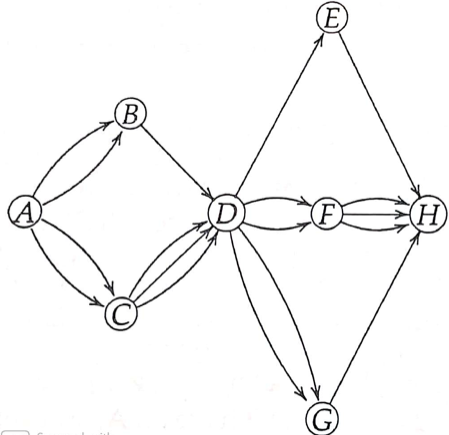
\includegraphics[width=0.5\linewidth]{Combinatoria/imgs/ciudadA_ciudadH}
		\caption{ Problema \ref{problema_ciudadA_ciudadH}. }
		\label{ciudadaciudadh}
	\end{figure}
	
	\item Yo tengo dos sombreros. En uno hay bolas numeradas del 1 al 15 y en el otro hay bolas numeradas del 16 al 25. Yo primero elijo un sombrero, luego, de ese sombrero elijo 3 bolas, sin devolver las bolas una vez son sacadas. Cuántas diferentes formas de seleccionar las balotas son posibles?. (2.2.2 de  \cite{ICP_Aops}). 
	
	\item Cuántas placas de carro se pueden hacer si deben ser de tres letras seguidas de dos números pares y luego 2 números impares?. (1.4.4 de \cite{ICP_Aops}).
	
	\item Cuántos números de 5 dígitos tienen al menos un 0 (un dígito cero)?. (2.3.2 de \cite{ICP_Aops}).
	
	\item Tengo 6 camisetas, 6 pantalones y 6 sombreros. Cada uno de ellos viene en los mismos colores (Es decir, dado un color hay un sombrero un pantalón y un sombrero de ese color). Si no me quiero vestir con las 3 prendas del mismo color . De cuántas formas diferentes me puedo vestir?. (2.2.3 de \cite{ICP_Aops}).
	
	\item De cuántas formas se pueden sentar 7 personas en una fila de sillas si dos de ellos, William y Cata no se quieren sentar juntos?. (2.3.4 de \cite{ICP_Aops}).
	
	\item De cuántas maneras se pueden organizar cinco libros en una biblioteca?. (1.4.5 de \cite{ICP_Aops}).
	
	\item Suponga que se tienen 6 libros diferentes, de los cuales dos son de matemáticas. De cuántas maneras se pueden organizar los seis libros en una repisa si se quiere que los libros de matemáticas queden cada uno en un extremo?. (1.4.6 de \cite{ICP_Aops}).
	
	\item Cuántos números de 3 dígitos no son múltiplos de 7?. (Capítulo 2.3 Problema 2.6 de \cite{ICP_Aops}).
	
	\item Hay 8 estudiantes en la final de las Olimpiadas Matemáticas. De cuántas formas puede quedar el podio si este consiste de un primer puesto, un segundo puesto y un tercer puesto?.
	
	\item De cuántas formas puedo arreglar 3 libros de matemáticas y 5 de historia en una biblioteca si necesito que haya un libro de matemáticas al inicio y al final?. (Capítulo 2.5 Problema 2.11 de \cite{ICP_Aops}).
	
	\item En una granja hay 4 gallinas, 2 perros y 5 gatos, de cuantas formas se pueden colocar los animales en una casa de mascota si los animales de la misma especie deben quedar adyacentes?. (2.5.2 de \cite{ICP_Aops}).
	
	\item La familia Ordoñez tiene 5 niños, 3 niñas y 2 de las niñas son gemelas. De cuántas formas se pueden sentar en una fila de 8 sillas si las gemelas insisten en quedar juntas y la otra hermana no quiere sentarse al lado de ninguna de ellas?. (2.5.3 de \cite{ICP_Aops}).
	
	\item (1.4.5 de \cite{ICP_Aops}). Simplificar las siguientes expresiones sin usar calculadora: 
	\begin{enumerate}
		\item $\frac{9!}{8!}$.
		\item $\frac{42!}{40!}$.
		\item $8!-7!$.
	\end{enumerate}
	
	\item En Bucaramanga juega una lotería que consiste de 25 balotas numeradas del 1 al 25. Las balotas se introducen en una urna. Cuatro balotas son sacadas una a la vez y sus números son registrados. El número ganador se compone de los cuatro números extraídos, en el orden que fueron sacados. Cuántos números ganadores pueden haber, si:
	\begin{enumerate}
		\item Cada balota una vez es retirada de la urna no se vuelve a ingresar.
		\item b)	Cada balota se vuelve a meter en la urna una vez es extraída y registrada, para así poder sacar la siguiente balota.
	\end{enumerate}
	
	\item \label{problema_triangulos_piramide_contar} (2.2.4 de \cite{ICP_Aops}). Cuántos triángulos aparecen en el diagrama \ref{trainguloscontar}.
	\begin{figure}
		\centering
		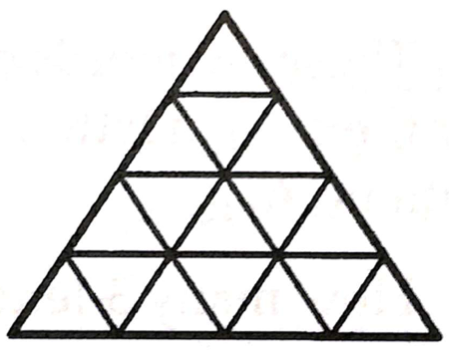
\includegraphics[width=0.5\linewidth]{Combinatoria/imgs/traingulos_contar}
		\caption{Problema \ref{problema_triangulos_piramide_contar}.}
		\label{trainguloscontar}
	\end{figure}
	
	\item \label{problema_circulo_seiscolores} Con seis colores se quiere pintar la bandera (Figura \ref{circulo4franjas}) de manera que no queden espacios adyacentes del mismo color. De cuántas maneras se puede pintar?
	\begin{figure}
		\centering
		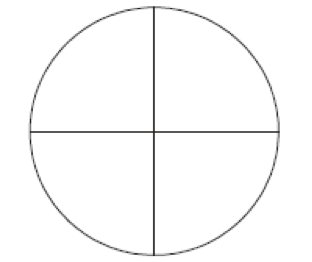
\includegraphics[width=0.4\linewidth]{Combinatoria/imgs/circulo_4_franjas}
		\caption{Problema \ref{problema_circulo_seiscolores}.}
		\label{circulo4franjas}
	\end{figure}
	
	\item Cuántas palabras de 3 letras pueden formarse si la segunda letra debe ser una vocal y la tercera letra debe ser distinta de la primera?.
	
	\item 40.	De cuántas formas es posible colocar 8 personas en una fila de modo que Camila y José no queden juntas y Marta y Martin si queden juntos?.
	
	\item 	Cuál es el máximo común divisor de 5!,10! Y 15!?. (1.33 de \cite{ICP_Aops}).
	
	\item De cuántas formas podemos colocar dos torres de ajedrez en el tablero de manera que ninguna amenace a la otra? (O sea que no estén en la misma fila ni en la misma columna).
	
	\item \textbf{Wow}. Cuántos enteros positivos menores que 500 se pueden expresar como la suma de dos cubos perfectos?.
	
	\item Juan, Carlos, Tomás, María y Jose van al cine y les fueron asignadas cinco sillas consecutivas. ¿De cuántas formas se pueden sentar, si Juan y María están uno al lado del otro y nadie, además de María, está junto a Juan?.
	
	\item Cuántos de los factoriales desde 1! Hasta 100! Son divisibles por 9?.
	
	\item Cuántos números naturales de 7 dígitos hay tales que tienen el dígito 4 exactamente tres veces y al dígito 8 exactamente dos veces?.
	
	\item Un candado de seguridad para una bicicleta necesita una clave de 5 dígitos. De cuántas formas se puede escoger la clave si debe ser un número impar, el dígito de la mitad debe ser par, el primer dígito debe ser múltiplo de 3, el segundo dígito debe ser un número primo? (Problema 2 \textit{UIS reto semanal bachillerato 2019}).
	
	\item \textbf{WOW}. Puede simplificar $P(n,k)P({n-k},j)$ donde $n,k$ y $j$ son enteros tales que $k\leq n$ y $j\leq {n-k}$?. (1.5.4 de \cite{ICP_Aops}).
	
	\item \textbf{WOW}. Cuál es el digito de las unidades de la suma $1!+2!+3!+\cdots+1000!?$. (1.35 de \cite{ICP_Aops}).
	
	\item \textbf{WOW}. De cuantas maneras se pueden elegir tres números del grupo de números 1,2,3,…100 de tal forma que el número más grande sea mayor que el producto de los otros dos? (el orden en que son sacados los números no importa). (2.4.5 de \cite{ICP_Aops}).
	
	\item Cuántos números de 4 dígitos tienen únicamente dígitos impares?. (2.16 de \cite{ICP_Aops}).
	
	\item Cuántas palabras de 3 letras pueden formarse con el alfabeto usual de 27 letras, si la primera letra debe ser una vocal?. (2.17 de \cite{ICP_Aops}).
	
	\item Cuántas claves de seguridad distintas se pueden formar con los dígitos del 1 al 5 si el segundo digito no puede ser el mismo que el primero y el tercero no puede ser el mismo que el segundo?. (2.18 de \cite{ICP_Aops}).
	
	\item Cuántas triplas (a,b,c) de números pares enteros positivos satisfacen $a^3+b^2+c\leq 50$?. (2.19 de \cite{ICP_Aops}).
	
	\item Cuántos números entre 100 y 200 no son cuadrados perfectos?. (2.20 de \cite{ICP_Aops}).
	
	\item Cuántos números de tres dígtios hay tales que el primer dígito es el triple que el tercer dígito?. (2.21 de \cite{ICP_Aops}).
	
	\item De cuantas formas se pueden sentar 6 niñas y 2 niños en una fila si los 2 niños insisten en sentarse juntos?. (2.22 de \cite{ICP_Aops}).
	
	\item Cuantos números de 4 dígitos tienen el segundo digito par y el cuarto digito al menos dos veces mayor que el segundo?. (2.23 de \cite{ICP_Aops}).
	
	\item Cuántos números de 3 digitos existen tales que la suma del digito de las centenas y el de las decenas es igual al de las unidades?. (2.26 de \cite{ICP_Aops}).
	
	\item La suma digital de un número es la suma de sus dígitos. Para cuantos números entre 24 y 125 incluyéndolos la suma digital es múltiplo de 7?. (2.27 de \cite{ICP_Aops}).
	
	\item \textbf{WOW.} Los $n$ miembros de un comité son numerados desde 1 hasta $n.$ Uno de los miembros es designado como el “cansón”. Los $n$ miembros se sientan en una fila de $n$ sillas, pero ningún miembro con un número mayor al del “cansón” se puede sentar inmediatamente a la derecha del “cansón”. Suponga que el “cansón” es el miembro $p$ con $1\leq p\leq n$. Encuentre una formula, en términos de $n$ y $p$, para el número de formas que se pueden sentar los miembros del comité. (2.29 de \cite{ICP_Aops}).
	
	\item \label{problema_tablaNOON} \textbf{WOW.} De cuántas formas usted puede deletrar la palabra NOON con la tabla \ref{tabla_NOON}? Usted puede empezar con cualquier letra, luego en cada paso usted se puede mover arriba, abajo, a la derecha, a la izquierda o en diagonal hasta que termine de deletrar la palabra. Usted no puede pasar por la misma casilla dos veces. (2.30 de \cite{ICP_Aops}).
	
	\begin{table}[]
		\centering
		\begin{tabular}{|l|l|l|l|}
			\hline
			N & N & N & N \\ \hline
			N & O & O & N \\ \hline
			N & O & O & N \\ \hline
			N & N & N & N \\ \hline
		\end{tabular}
		\caption{Problema \ref{problema_tablaNOON}.}
		\label{tabla_NOON}
	\end{table}
	
	\item Un número palíndromo es un número que se lee igual de derecha a izquierda que de izquierda a derecha, por ejemplo 12321. (2.31 de \cite{ICP_Aops}).
	\begin{enumerate}
		\item Cuántos números palíndromos hay de 4 digitos?
		\item Cuántos números palíndromos hay de 5 digitos?
		\item \textbf{Wow} Cuántos números palíndromos hay de $n$ digitos?
		\item \textbf{Woww}. Suponga que hacemos una lista con los números palíndromos de k dígitos que están formados únicamente con los dígitos 8 y 9, y además tiene al menos un 8 y al menos un 9. Cuál es el valor más pequeño de k tal que hayan al menos 2019 números en la lista? 
	\end{enumerate}
	
	\item Sea $S$ un cubo. Calcule cuantos planos pasan a través de al menos 3 vértices de $S$. (2.32 de \cite{ICP_Aops}).
	
	\item \textbf{Woww}. Cuantos ceros se escriben al escribir todos los enteros desde 1 hasta 256 en binario?. (2.33 de \cite{ICP_Aops}).
	
	\item Cuántas palabras de 5 letras (donde cualquier lista de 5 letras se considera una palabra) tienen al menos dos letras iguales consecutivas?. (2.34 de \cite{ICP_Aops}).
	
	\item Un número entero positivo es llamado \textit{"estable"} si al menos uno de sus dígitos tiene el mismo valor que su posición en el número. Por ejemplo, $78247$ es estable debido a que un 4 aparece en la 4ta posición. Cuántos números estables de tres dígitos hay?. (Ejercicio 26 de \textit{XXIX Competencia Regional de Matemáticas,Nivel Intermedio UAN 2019}). 
\end{enumerate}
\newpage


\chapter{Principio de Inclusión y Exclusión}\label{Pinclusionyexclusion}
\vspace{3cm}

(***importante aclarar conjuntos....la diferencia entre ``y" y la ``o".)
\vspace{3cm}




\newpage
\begin{center}
	\vspace{-1cm}
	\section{ Ejercicios: Principio de Inclusión y Exclusión}
\end{center}	
\begin{enumerate}
	\item En un colegio hay 170 estudiantes. Algunos de ellos asisten a la lúdica de Club matemático,  cine o fútbol, que se realizan por las tardes. Se sabe que
	\begin{itemize}
		\item 65 estudiantes asisten a Club matemático.
		\item 96 asisten a cine.
		\item 94 asisten a fútbol.
		\item 35 estudiantes asisten únicamente a la lúdica de cine.
		\item 42 asisten a cine y fútbol.
		\item 40 asisten a Club matemático y fútbol.
		\item 22 estudiantes asisten a las tres lúdicas.
	\end{itemize}
	Con base en la información anterior,
	\begin{enumerate}
		\item ¿Cuántos estudiantes están únicamente en el Club matemático?
		\item ¿Cuántos están únicamente en cine?
		\item ¿Cuántos de ellos asisten a cine o fútbol?
		\item ¿Cuántos asisten por lo menos a una de las lúdicas?
		\item ¿Cuántos estudiantes no asisten a ninguna lúdica?
	\end{enumerate}
\end{enumerate}
\newpage
